\section[Bagging and Random Forests]{Bagging and Random Forests}

\subsection[Introduction]{Introduction}

\begin{frame}{Motivation for Bagging}
	\begin{itemize}
		\item We previously observed that CART can lead to overfitting when its hyperparameters (minimum leaf size, minimum entropy, maximum depth) are tuned too aggressively.
		\item Conversely, overly conservative settings can result in underfitting.
		\item Although it is possible to tune these parameters to achieve a satisfying trade-off, we will explore an alternative approach: \textbf{bagging} (bootstrap aggregating).
		\item Combining CART with bagging gives rise to a powerful new algorithm: \textbf{Random Forests}!
	\end{itemize}
\end{frame}

\begin{frame}{General Idea of Bagging}
	The core principle of Bagging can be summarized in the following points:
	\begin{itemize}
		\item We generate $B$ resampled datasets from the original training data using the bootstrap algorithm.
		\pause
		\item On each bootstrap sample, we train a decision tree with aggressive settings, intentionally accepting high variance. Our primary goal here is to minimize bias.
		\pause
		\item To counteract the risk of overfitting resulting from this choice, when making a prediction, all trained trees output their individual predictions, and these predictions are \textbf{averaged}.
		\pause
		\item Bagging belongs to the family of \textbf{ensemble methods} in machine learning.
	\end{itemize}
\end{frame}

\subsection[Algorithm]{Algorithm}

\begin{frame}{Specific Feature of Random Forests}
	In addition to Bagging, Random Forests introduce an extra subtlety. Within the CART algorithm, during the multi-dimensional step, we no longer explore \textbf{all} available input features, but rather a \textbf{random subset}:
	\begin{itemize}
		\item We replace Step 1: "For each $j \in \llbracket 1;d \rrbracket$, apply the one-dimensional algorithm considering feature $X_j$."
		\item With:
		\begin{enumerate}
			\item Determine the number of features to consider, typically $d^* = \lfloor \sqrt{d} \rfloor$.
			\item Randomly select features by drawing $d^*$ samples without replacement from the set of all available features $\{1, 2, \cdots, d\}$.
		\end{enumerate}
	\end{itemize}
\end{frame}

\begin{frame}{Decision Making}
	To compute a prediction on inference data $x_i$, we query the $B$ generated trees and average their outputs. If we denote by $P_k^{(b)}(x_i) \in [0, 1]$ the probability predicted by tree $b$ for class $k$ given the input $x_i$, then the prediction made by the Bagging algorithm is:
	\begin{equation}
		P_k(x_i) = \frac{1}{B} \sum_{b=1}^B P_k^{(b)}(x_i)
		\nonumber
	\end{equation}
	This averaging operation is what reduces the variance introduced by each individual tree in the Random Forest. It is known as \textbf{Soft voting}.
\end{frame}


\subsection[Case Study]{Case Study}

\begin{frame}{MNIST Handwritten Digits}
	We will use the MNIST dataset as our benchmark, which was introduced in the course on Principal Component Analysis and contains grayscale images of handwritten digits: \href{https://www.kaggle.com/datasets/hojjatk/mnist-dataset}{\textbf{Kaggle MNIST Dataset}}.
	\begin{itemize}
		\item Yann LeCun, Courant Institute, NYU
		\item Corinna Cortes, Google Labs, New York
		\item Christopher J.C. Burges, Microsoft Research, Redmond
	\end{itemize}
\end{frame}

\begin{frame}{Simplification and Algorithms}
	We will train a Random Forest on this MNIST data using a simplified version of the features obtained via Principal Component Analysis.
	
	\vspace{0.5cm}
	
	The Scikit-Learn algorithms we will utilize:
	\begin{itemize}
		\item \href{https://scikit-learn.org/stable/modules/generated/sklearn.decomposition.PCA.html}{\texttt{sklearn.decomposition.PCA}}
		\item \href{https://scikit-learn.org/stable/modules/generated/sklearn.tree.DecisionTreeClassifier.html}{\texttt{sklearn.tree.DecisionTreeClassifier}}
		\item \href{https://scikit-learn.org/stable/modules/generated/sklearn.ensemble.RandomForestClassifier.html}{\texttt{sklearn.ensemble.RandomForestClassifier}}
	\end{itemize}
\end{frame}

\begin{frame}{Multi-Class Classification}
	We are now facing a multi-class classification problem. This requires a few adjustments to the performance metrics we previously encountered:
	\begin{itemize}
		\item Confusion matrix: $C$.
		\item ROC curve: $\mathcal{C}_{\text{ROC}}$.
		\item Area Under the ROC Curve: $\operatorname{AUC}$.
	\end{itemize}
\end{frame}

\begin{frame}{Multi-Class Classification: Confusion Matrix}
	The definition introduced in the first chapter remains applicable:
	\begin{block}{Definition: Confusion Matrix}
		In a $K$-class classification problem, the confusion matrix $C \in \mathcal{M}_{K,K}$ is defined as follows, based on the \textbf{true} classes $y^{(i)}$ and the \textbf{predicted} classes $\hat{y}^{(i)}$ for each observation $i$:
		\begin{equation}
			C_{m,n} = \operatorname{card} \left( \{i \in \{1, 2, \cdots, N\}\} \mid y^{(i)} = m \, \text{and} \, \hat{y}^{(i)} = n \right)
			\nonumber
		\end{equation}
	\end{block}
	\vspace{0.5cm}
	\pause
	The key difference is that we can no longer directly map the matrix elements of $C$ to unique global values of \textbf{true positives}, \textbf{false positives}, \textbf{true negatives}, and \textbf{false negatives}.
\end{frame}

\begin{frame}{Multi-Class Classification: One-vs-Rest Strategy}
	A general approach consists of computing these rates ($\operatorname{TP}$, $\operatorname{FP}$, $\operatorname{TN}$, $\operatorname{FN}$) for each individual class $k$ using a One-vs-Rest strategy:
	
	\begin{equation}
		\begin{aligned}
			\operatorname{TP}_k &= \operatorname{card} \left( \{i \in \{1, 2, \cdots, N\}\} \mid y^{(i)} = k \, \text{and} \, \hat{y}^{(i)} = k \right) \\
			\operatorname{FP}_k &= \operatorname{card} \left( \{i \in \{1, 2, \cdots, N\}\} \mid y^{(i)} \ne k \, \text{and} \, \hat{y}^{(i)} = k \right) \\
			\operatorname{TN}_k &= \operatorname{card} \left( \{i \in \{1, 2, \cdots, N\}\} \mid y^{(i)} \ne k \, \text{and} \, \hat{y}^{(i)} \ne k \right) \\
			\operatorname{FN}_k &= \operatorname{card} \left( \{i \in \{1, 2, \cdots, N\}\} \mid y^{(i)} = k \, \text{and} \, \hat{y}^{(i)} \ne k \right)
		\end{aligned}
		\nonumber
	\end{equation}
	
\end{frame}

\begin{frame}{Multi-Class Classification: ROC Curve in One-vs-Rest Strategy}
	Using these new definitions, we can define a True Positive Rate $\operatorname{TPR}_k$ and a False Positive Rate $\operatorname{FPR}_k$ specifically for class $k$:
	\begin{equation}
		\begin{cases}
			\operatorname{TPR}_k = \displaystyle \frac{\operatorname{TP}_k}{\operatorname{TP}_k + \operatorname{FN}_k} \\[10pt]
			\operatorname{FPR}_k = \displaystyle \frac{\operatorname{FP}_k}{\operatorname{FP}_k + \operatorname{TN}_k}
		\end{cases}
		\nonumber
	\end{equation}
	\pause
	This allows us to formulate a definition for the class-specific ROC curve:
	\begin{block}{Definition: One-vs-Rest ROC Curve}
		For a given class $k$, the ROC curve, denoted by $\mathcal{C}_{\text{ROC},k}$, represents the relationship between the True Positive Rate $\operatorname{TPR}_k$ and the False Positive Rate $\operatorname{FPR}_k$ as the decision threshold $\theta$ varies:
		\begin{equation}
			\mathcal{C}_{\text{ROC},k} = \{ \left(\operatorname{FPR}_k, \operatorname{TPR}_k\right) \in [0, 1]^2 \mid \theta \in [0, 1]\}
			\nonumber
		\end{equation}
	\end{block}
\end{frame}

\begin{frame}{Multi-Class Classification: AUC in One-vs-Rest Strategy}
	Finally, the Area Under the ROC Curve for class $k$, denoted as $\operatorname{AUC}_k$, can be defined as a function of the decision threshold $\theta \in [0, 1]$, where $t \in [0, 1]$ represents the False Positive Rate for a given value of $\theta$, meaning $t = \operatorname{FPR}_k(\theta)$:
	\begin{block}{Definition: One-vs-Rest AUC}
		For a given class $k$, the Area Under the ROC Curve, denoted by $\operatorname{AUC}_k$, is defined as:
		\begin{equation}
			\operatorname{AUC}_k = \int_{t = 0}^{t = 1} \operatorname{TPR}_k(t) dt
			\nonumber
		\end{equation}
	\end{block}
\end{frame}

\begin{frame}{Example Results}
	Here is an example result obtained on the MNIST dataset using a Random Forest classifier:
	\begin{columns}
		\begin{column}{0.5\textwidth}
			\begin{figure}
				\centering
				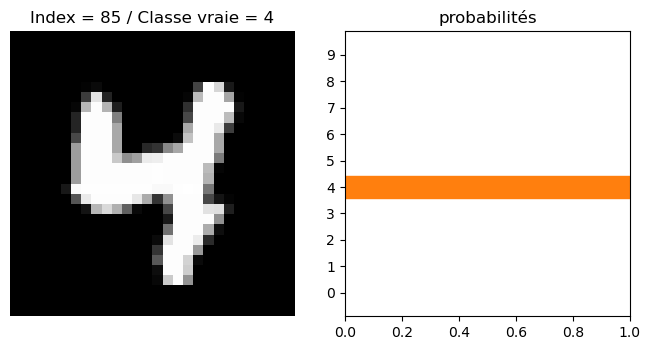
\includegraphics[width=1.0\linewidth]{Images/MNIST_1}
				\label{fig:MNIST_1}
			\end{figure}			
		\end{column}
		\begin{column}{0.5\textwidth}
			\begin{figure}
				\centering
				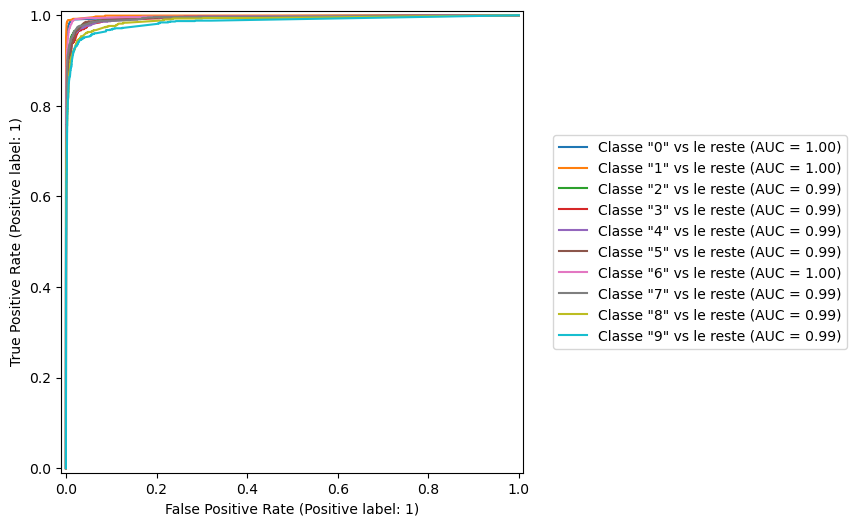
\includegraphics[width=1.0\linewidth]{Images/MNIST_2}
				\label{fig:MNIST_2}
			\end{figure}			
		\end{column}
	\end{columns}	
\end{frame}

\subsection[Summary]{Summary}

\begin{frame}{Random Forests (Bagging)}
	\begin{figure}
		\centering
		\resizebox{0.95\textwidth}{!}{
			\begin{tikzpicture}[
				>=stealth,
				node distance=1.5cm and 2.5cm,
				data/.style={rectangle, rounded corners, draw=black, fill=blue!10, minimum width=2.5cm, minimum height=1cm, align=center},
				tree/.style={rectangle, draw=black, fill=green!15, minimum width=2.5cm, minimum height=1cm, align=center},
				agg/.style={rectangle, rounded corners, draw=black, fill=orange!20, minimum width=3cm, minimum height=1cm, align=center},
				arrow/.style={thick, ->}
				]
				
				% Nodes
				\node[data] (D) {Data $\mathcal{D}$};
				\node[tree] (T2) [right=3cm of D] {Tree 2\\(Deep)};
				\node[tree] (T1) [above=0.5cm of T2] {Tree 1\\(Deep)};
				\node[tree] (T3) [below=0.5cm of T2] {Tree $B$\\(Deep)};
				\node[agg] (Vote) [right=2cm of T2] {Average\\(Soft voting)};
				\node (Out) [right=1.5cm of Vote] {\textbf{Prediction}};
				
				% Arrows
				\draw[arrow] (D) -- node[above, sloped, midway, font=\footnotesize] {Bootstrap 1} (T1.west);
				\draw[arrow] (D) -- node[above, midway, font=\footnotesize] {Bootstrap 2} (T2.west);
				\draw[arrow] (D) -- node[below, sloped, midway, font=\footnotesize] {Bootstrap $B$} (T3.west);
				
				\draw[arrow] (T1.east) -- (Vote.west);
				\draw[arrow] (T2.east) -- (Vote.west);
				\draw[arrow] (T3.east) -- (Vote.west);
				
				\draw[arrow] (Vote) -- (Out);
				
				% Variables
				\node[text=green!40!black, font=\footnotesize, align=center] at (5.5, 2.5) {\textit{Random subsets}\\\textit{of $d^*$ features}\\\textit{at each split}};
				
			\end{tikzpicture}
		}
	\end{figure}
	\vspace{0.5cm}
	\textbf{Parallel} architecture. We reduce the \textbf{variance} of complex and independent trees.
\end{frame}